\documentclass[letter]{article}
\usepackage{anysize}
\usepackage[spanish]{babel}
\usepackage{graphicx}
\usepackage[utf8]{inputenx}
\usepackage{listings}
\usepackage{ulem}
\usepackage{verbatim}
\usepackage{xcolor}

\usepackage{color}
\definecolor{gray}{rgb}{0.4,0.4,0.4}
\definecolor{darkblue}{rgb}{0.0,0.0,0.6}
\definecolor{cyan}{rgb}{0.0,0.6,0.6}

\marginsize{2cm}{2cm}{2cm}{2cm} %{izq}{der}{top}{bottom}

\lstset{tabsize=2,language=java,basicstyle=\scriptsize\ttfamily,numberstyle=\scriptsize\ttfamily,numbers=left,aboveskip={1.5\baselineskip},columns=fixed,showstringspaces=false,extendedchars=true,breaklines=true,prebreak = \raisebox{0ex}[0ex][0ex]{\ensuremath{\hookleftarrow}},frame=single,showtabs=false,showspaces=false,showstringspaces=false,identifierstyle=\color[rgb]{0,0,0},keywordstyle=\color[rgb]{0,0,1},commentstyle=\color[rgb]{0,0.55,0},stringstyle=\color[rgb]{1,0,0},language=java}

\lstset{
  basicstyle=\ttfamily,
  columns=fullflexible,
  showstringspaces=false,
  commentstyle=\color{gray}\upshape
}

\lstdefinelanguage{xml}
{
  morestring=[b]",
  morestring=[s]{>}{<},
  morecomment=[s]{<?}{?>},
  stringstyle=\color{black},
  identifierstyle=\color{darkblue},
  keywordstyle=\color{cyan},
  morekeywords={xmlns,version,type}% list your attributes here
}

% ------------- preambulo -------------

\setlength{\parindent}{0in}
\setlength{\textheight}{9in}
\setlength{\parskip}{0.25in}

\begin{document}

% ------------ portada ---------------

\thispagestyle{empty}
\begin{flushleft}
  Universidad de Chile\\Facultad de Ciencias Físicas y Matemáticas\\Departamento de Ciencias de la Computación\\[4cm]
\end{flushleft}
\begin{center}
  \huge{Aplicaciones Empresariales sobre la Plataforma Java J2EE\\[1.5cm] CC5604-1\\[0.4cm]}
  \Large{\textbf{Informe de proyecto Fase 2\\[2.5cm]}José Manuel Tapia González\\[0.4cm]René Fernando Tapia Pincheira\\[2.5cm] \today}
\end{center}

%-----------indice---------------------------

\newpage
\tableofcontents

%-----------introduccion---------------------

\newpage
\section{Introducción}

A grandes rasgos, el problema propuesto consiste en crear una aplicación web administrativa para el FC Barcelona (nuestro cliente), el cual en esta segunda etapa, desea crear la capa de presentación de la aplicación. La aplicación debe proveer una interfaz gráfica para las funcionalidades implementadas en la entrega anterior (mantención de usuarios, activos, pasivos, socios, personal, etc.)

Además se deben respetar directrices generales, como por ejemplo, usar servlet/jsp, implementar filtros, mecanismos de seguridad, entre otros.

Para resumir lo explicado en el informe de la entrega anterior, recordemos que la aplicación fue implementada usando el framework \texttt{Spring}, \texttt{Spring-MVC} y \texttt{Hibernate}, además de contar con tests escritos usando \texttt{JUnit}. Se utilizó el editor \texttt{Intellij IDEA}, \texttt{JDK 6} y sistema operativo \texttt{Windows 7}.

%-----------enunciado del problema-----------
\newpage
\section{El problema}

Podemos dividir el problema en varias tareas.
\begin{itemize}
\item Implementar login de usuarios y filtro de acceso a recursos.

 Para esta tarea, se usó el módulo \texttt{Spring security}, ya que ofrecía exactamente la funcionalidad pedida y se integraba perfectamente con el resto de la aplicación (que ya utilizaba spring desde antes). Las particularidades de cada página se analizaron e implementaron por separado, haciendo especial énfasis en que la aplicación sea fácil e intuitiva para el usuario.

\item Programar página de administración de activos, socios, contratos, pasivos, personal y usuarios.

En general, estas páginas siguen un modelo estándar para agregar, borrar y actualizar elementos. Se utilizó la librería \texttt{DisplayTag} para listar los elementos en base de datos. Se utilizó \texttt{JQuery} y \texttt{JQuery-Ui} para la interfaz de usuario (selector de fechas, diálogos modales, botones, ajax, etc).

\item Programar página de resumen de finanzas.

Esta pantalla es similar a los administradores, pero más simple, solo listando el resultado de una consulta sobre los activos y pasivos.

\item Preparar script para empaquetado de aplicación.

Se utilizó \texttt{Ant} para compilar, correr los tests y empaquetar la aplicación. Es necesario desplegar manualmente la aplicación (\texttt{.ear}), ya que es particularmente díficil compatibilizar esta acción a través de los distintos servidores de aplicaciones.

\end{itemize}

%-------- solucion --------------------------
\newpage
\section{Solución del problema}

A continuación se explica en detalle como está implementada cada tarea listada anteriormente.

\subsection{Login de usuarios}

Como se adelantó anteriormente, se utilizó el módulo de seguridad del framework \texttt{Spring}. Para esto fue necesario agregar las librerías \texttt{.jar} al buildpath y classpath del proyecto. Luego fue necesario agregar las siguientes definiciones en el archivo \texttt{web.xml}:

\begin{lstlisting}[language=xml]
 <filter>
  <filter-name>springSecurityFilterChain</filter-name>
  <filter-class>org.springframework.web.filter.DelegatingFilterProxy</filter-class>
 </filter>
 <filter-mapping>
  <filter-name>springSecurityFilterChain</filter-name>
  <url-pattern>/*</url-pattern>
 </filter-mapping>
\end{lstlisting}

De esta forma se pasan todas las urls de la aplicación a través del filtro definido por los parámetros a continuación. Luego en el fichero de configuración \texttt{applicationContext.xml} (también conocido como \texttt{beans.xml} o \texttt{spring.xml}) definimos la seguridad de nuestra aplicación. A continuación los patrones de las urls que pueden ser accesadas libremente (sin autenticación):

\begin{lstlisting}[language=xml]
 <s:http pattern="/images/**" security="none" />
 <s:http pattern="/js/**" security="none" />
 <s:http pattern="/css/**" security="none" />
 <s:http pattern="/login.html" security="none" />
 <s:http pattern="/403.html" security="none" />
 <s:http pattern="/404.html" security="none" />
\end{lstlisting}
A continuación indicamos algunos parámetros. Todo el resto de las urls requieren autenticación, la página default de acceso denegado (error 403), y un hook en el proceso general de autenticación (un custom filter, que es llamado luego del envío de parámetros desde el formulario, para validar el ingreso del captcha):
\begin{lstlisting}[language=xml]
<s:http auto-config="false" access-denied-page="/403.html" entry-point-ref="entryPoint" >
  <s:custom-filter ref="authenticationFilter" position="FORM_LOGIN_FILTER"/>
  <s:logout logout-url="/logout" logout-success-url="/login.html"/>
  <s:intercept-url pattern="/**" access="isAuthenticated()"/>
  ...
</s:http>
<bean id="entryPoint" class="org.springframework.security.web.authentication.LoginUrlAuthenticationEntryPoint">
 <property name="loginFormUrl" value="/login.html"/>
</bean>
\end{lstlisting}

El custom filter mencionado anteriormente se encarga de la validación de usuarios. Con un \texttt{authenticationManager} indicamos el bean que recuperará el usuario desde la base de datos que ha ingresado sus credenciales (incluído su password), para que el framework decida si debe permitir el ingreso o no. También define las acciones a seguir en caso de login incorrecto, por ejemplo.

\begin{lstlisting}[language=xml]
 <bean id="authenticationFilter" class="cl.cc5604.fcbarcelonaonline.business.application.ExUsernamePasswordAuthenticationFilter">
  <property name="filterProcessesUrl" value="/loginProcess"/>
  <property name="authenticationManager" ref="theAuthenticationManager"/>
  <property name="successHandler" ref="customAuthenticationSuccessHandler"/>
  <property name="failureHandler" ref="customAuthenticationFailureHandler"/>
 </bean>

 <s:authentication-manager alias="theAuthenticationManager">
  <!-- clase anotada, inyectada por spring -->
  <s:authentication-provider user-service-ref="securityUserDetailsService"/>
 </s:authentication-manager>

    <!-- bean 2: set the default failure url here -->
 <bean id="customAuthenticationFailureHandler" class="org.springframework.security.web.authentication.SimpleUrlAuthenticationFailureHandler">
  <property name="defaultFailureUrl" value="/login.html?error=true" />
 </bean>

 <!-- bean 3: set the default target url here -->
 <bean id="customAuthenticationSuccessHandler" class="org.springframework.security.web.authentication.SimpleUrlAuthenticationSuccessHandler">
  <property name="defaultTargetUrl" value="/app/main/index.html" />
 </bean>
\end{lstlisting}
El custom filter, básicamente, recupera la respuesta del captcha desde la sesión del usuario y la compara con el campo que ha ingresado el usuario en el formulario de login (al generar la imagen para el captcha, ese servlet guardó la respuesta en la sesión de la request que recibió). Luego almacena en una variable thread local el estado de la validación, para que posteriormente el authenticationManager rechace la conexión, si el código no coincide:
\begin{lstlisting}
public class ExUsernamePasswordAuthenticationFilter extends UsernamePasswordAuthenticationFilter {
 ...
 @Override
 public Authentication attemptAuthentication(HttpServletRequest request, HttpServletResponse response) throws AuthenticationException {
  HttpSession session = request.getSession(true); // get session
  String errorMsg = null;

  // get previously stored response (set by CageCaptchaServlet)
  Object objCaptchaResponse = session.getAttribute(CageCaptchaServlet.CAPTCHA_RESPONSE);
  // input from form submit
  String captchaCode = request.getParameter(CageCaptchaServlet.CAPTCHA_CODE); 
  String captchaResponse = (objCaptchaResponse == null ? null : String.valueOf(objCaptchaResponse));

  // perform validation of captcha
  if (captchaCode == null || captchaResponse == null) {
   errorMsg = "Invalid session.";
  } else if (!captchaCode.equals(captchaResponse)) {
   errorMsg = "Invalid captcha.";
  }

  // store status of validation for later exception
  ThreadLocal<String> threadLocal = CaptchaSingleton.getInstance().getThreadLocal();
  threadLocal.set(errorMsg);

  return super.attemptAuthentication(request, response);
 }
}
\end{lstlisting}
Más adelante, en una etapa posterior de la cadena de filtros del mecanismo de seguridad, se aplica el resultado de la validación del captcha, así como se recupera el usuario cuya password será validada internamente por el framework. El método implementado en la siguiente clase, es llamado por el framework. Aquí se puede rechazar la conexión si el captcha era inválido, si el usuario no existe, etc:
\begin{lstlisting}
@Service(value = "securityUserDetailsService")
public class SecurityUserContextLoader implements UserDetailsService {
...
    @Override
    @Transactional
    public UserDetails loadUserByUsername(String username) throws UsernameNotFoundException, DataAccessException {
        // retrieve error in captcha mechanism
        ThreadLocal<String> threadLocal = CaptchaSingleton.getInstance().getThreadLocal();
        String errorMsg = threadLocal.get();
        if (errorMsg != null) {
            throw new BadCredentialsException(errorMsg);
        }

        // user credential mechanism
        UserEntity userEntity = userAdministration.findByUsername(username);
        if (userEntity == null) {
            throw new BadCredentialsException("Acceso denegado");
        }

        return new User(userEntity.getUsername(), userEntity.getPassword(), true, true, true, true, new LinkedList<GrantedAuthority>());
    }
}
\end{lstlisting}

Finalmente, el login de usuarios, que es el punto de entrada de la aplicación\footnote{\texttt{http://localhost:7001/fcbarcelonaonline/login.html}}, se ve en la siguiente imagen:

\begin{figure}
  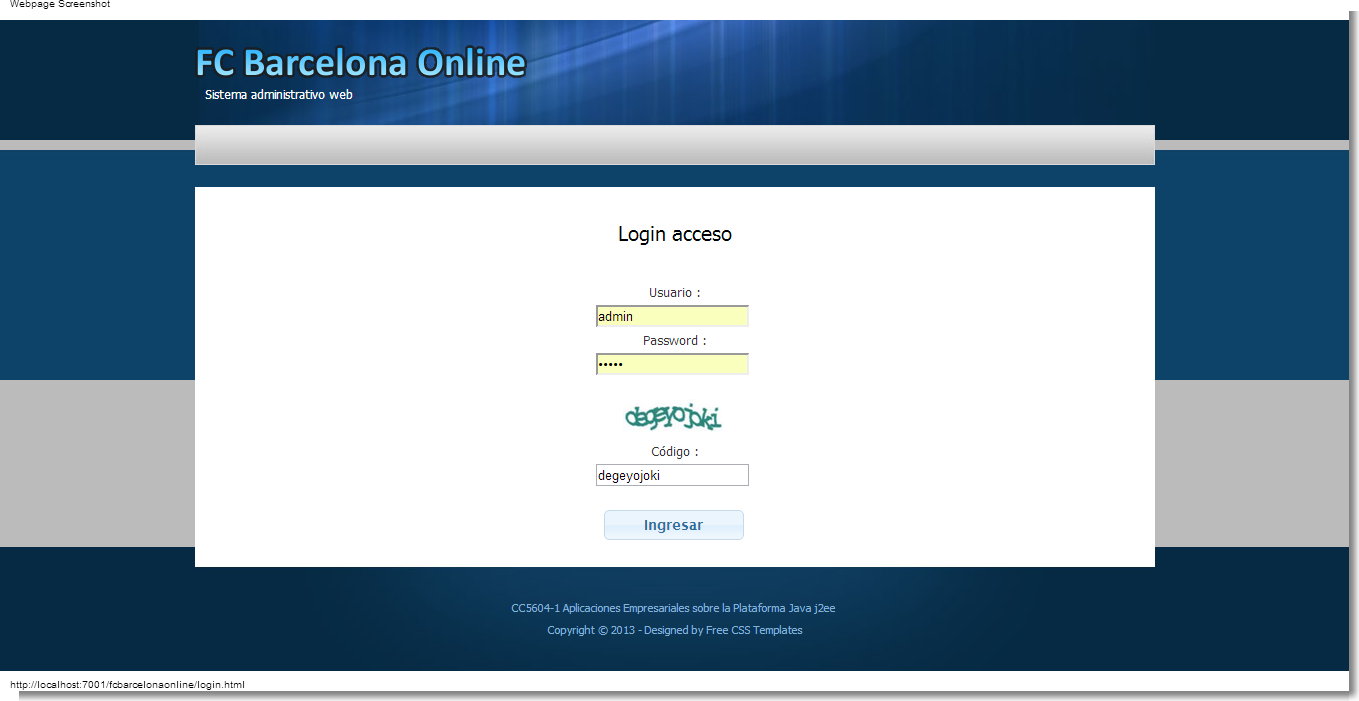
\includegraphics[width=\textwidth]{figs/fig1.png}
\caption{Página de ingreso de credenciales de la aplicación.}
\end{figure}

\subsection{Administradores.}
Para simplificar la explicación, se usará como modelo el administrador de usuarios, pues el resto es similar. Básicamente, cada controlador tiene una url mapeada, y estas urls comparten el prefijo \texttt{app}\footnote{\texttt{http://localhost:7001/fcbarcelonaonline/app/*}}. Veamos paso a paso como se configuró la aplicación para usar controladores de \texttt{Spring-MVC}.

Primero se descargaron las librerías y sus dependencias y se agregaron al buildpath y classpath del proyecto. La primera configuración se realizó en \texttt{web.xml}. Aquí especificamos el dispatcher usado para los controladores y como éstos deben localizar los recursos \texttt{.jsp} para desplegar al usuario.

\begin{lstlisting}[language=xml]
 <servlet>
  <servlet-name>mvc-dispatcher</servlet-name>
   <servlet-class>org.springframework.web.servlet.DispatcherServlet</servlet-class>
   <load-on-startup>1</load-on-startup>
  </servlet>
  <servlet-mapping>
   <servlet-name>mvc-dispatcher</servlet-name>
   <url-pattern>/app/*</url-pattern>
  </servlet-mapping>
 <context-param>
  <param-name>contextConfigLocation</param-name>
  <param-value>WEB-INF/mvc-dispatcher-servlet.xml</param-value>
 </context-param>
 <listener>
  <listener-class>org.springframework.web.context.ContextLoaderListener</listener-class>
 </listener>
\end{lstlisting}
El archivo que especifica el \texttt{RequestDispatcher} no es más que una extensión del archivo \texttt{applicationContext.xml}. Aquí indicamos el prefijo y sufijo de los recursos que serán desplegados (en este caso el prefijo es la ruta base donde están todos los \texttt{.jsp} de la aplicación, y el sufijo, la extensión de las vistas).
\begin{lstlisting}[language=xml]
<beans ...>
<bean id="viewResolver" class="org.springframework.web.servlet.view.InternalResourceViewResolver">
   <property name="prefix"><value>/WEB-INF/pages/</value></property>
   <property name="suffix"><value>.jsp</value></property>
</bean>
...
</beans>
\end{lstlisting}

Hecho esto, basta agregar una clase anotada que implemente la lógica de presentación y haga las llamadas a lógica de negocio (que convenientemente se inyecta a través de \texttt{Spring}).

\begin{lstlisting}
package cl.cc5604.fcbarcelonaonline.controller;
... // imports
@Controller
@RequestMapping("/user")
public class UserController {
...
    @Autowired private IUserAdministration userAdministration;

    @RequestMapping("/index.html")
    public ModelAndView index() {
        return new ModelAndView("frame")
                .addObject("availableUser", userAdministration.findAllUsers())
                .addObject("module", 7);
    }
...
    @RequestMapping(value = "/handlePost", method = RequestMethod.POST)
    public View handlePost(
            @RequestParam("id") String id,
            @RequestParam("username") String username,
            @RequestParam("password") String password,
            @RequestParam("passwordConfirm") String passwordConfirm,
            HttpServletRequest request,
            HttpServletResponse response
    ) {
      // handle post
    }
...
}
\end{lstlisting}

A continuación se incluyen imágenes representativas de la aplicación (también de la página de resumen de finanzas).

\begin{figure}
\centering
  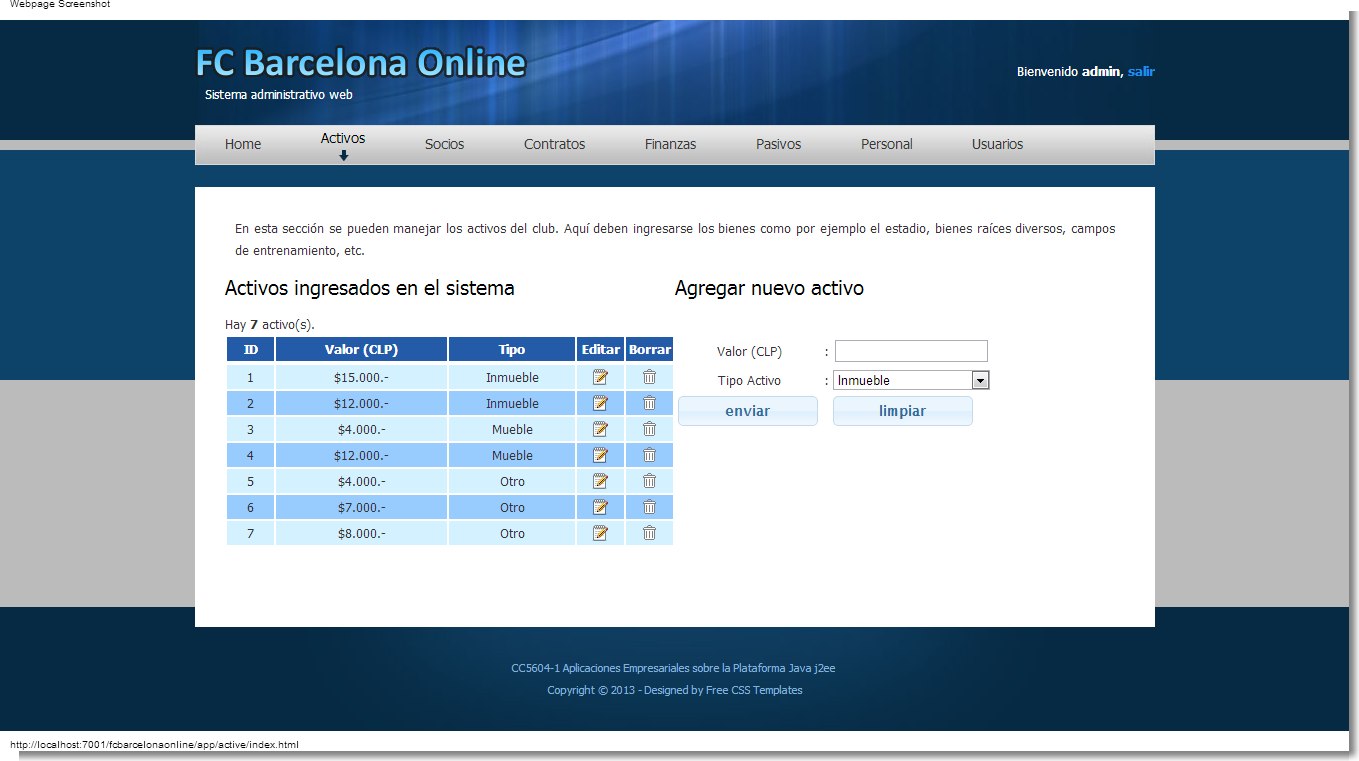
\includegraphics[width=\textwidth]{figs/fig2.png}
  \caption{Administración de activos del club.}
\end{figure}

\begin{figure}
\centering
  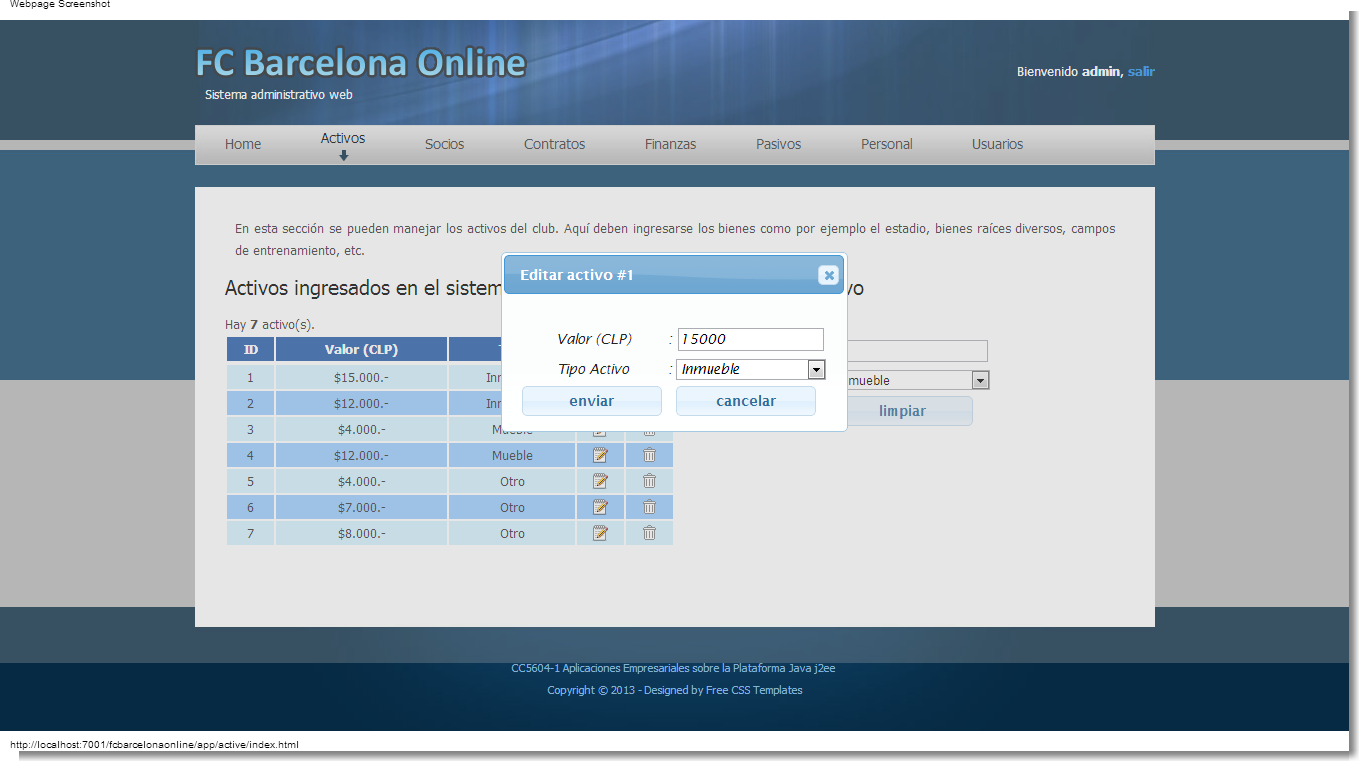
\includegraphics[width=\textwidth]{figs/fig3.png}
  \caption{Diálogo modal para la edición de un item de la lista de activos.}
\end{figure}

\begin{figure}
\centering
  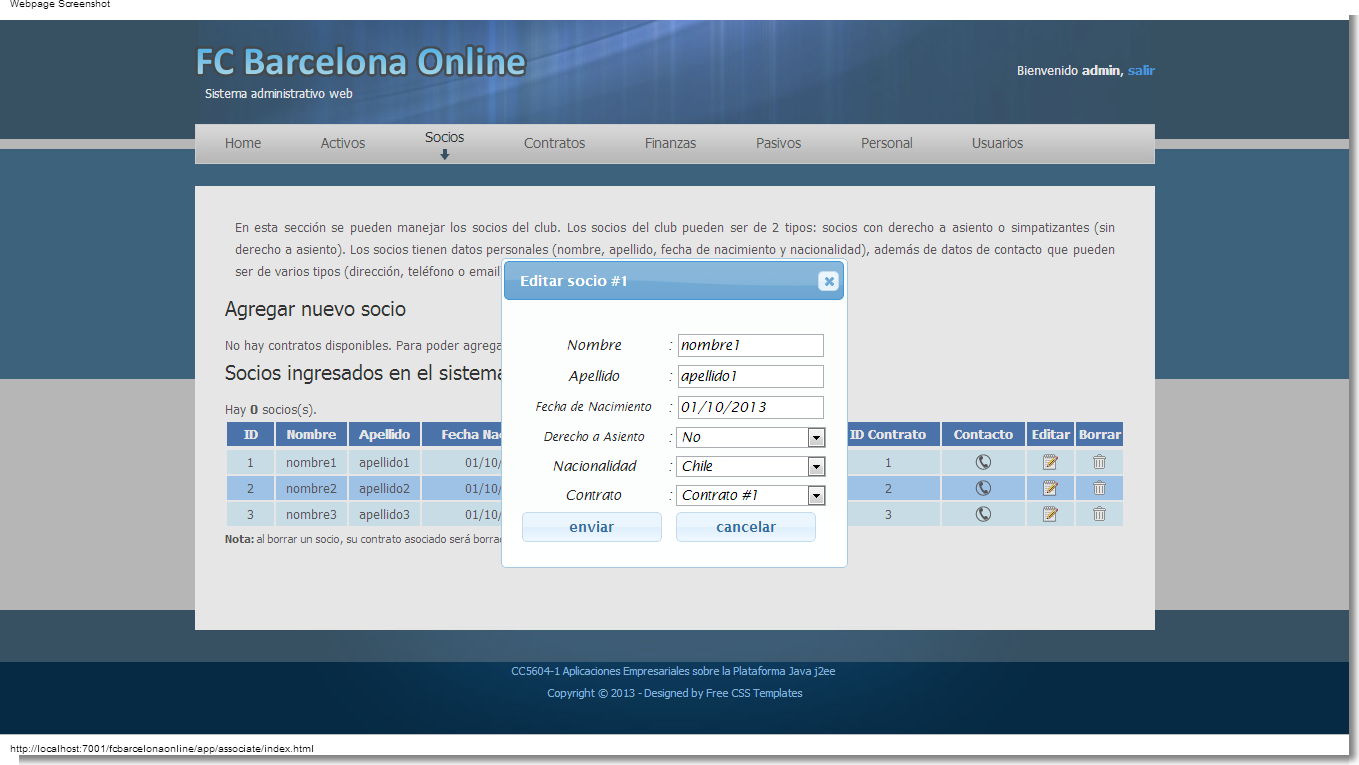
\includegraphics[width=\textwidth]{figs/fig4.png}
  \caption{Diálogo modal para la edición de un item de la lista de socios. Notar como se despliegan las nacionalidades y contratos disponibles (entidades recuperadas desde la base de datos).}
\end{figure}

\begin{figure}
\centering
  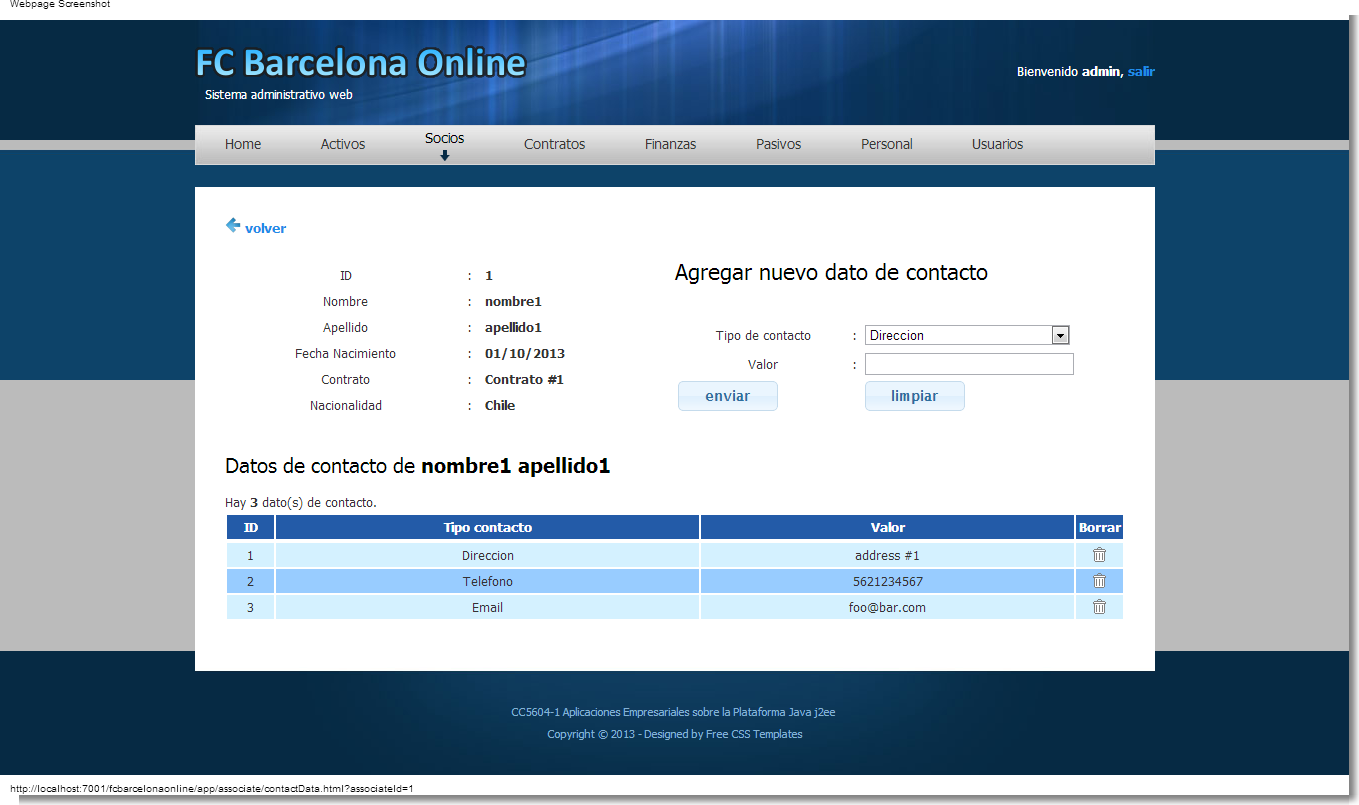
\includegraphics[width=\textwidth]{figs/fig5.png}
  \caption{La administración de socios también contempla la edición de datos de contacto. La pantalla es similar al resto de los administradores.}
\end{figure}

\begin{figure}
\centering
  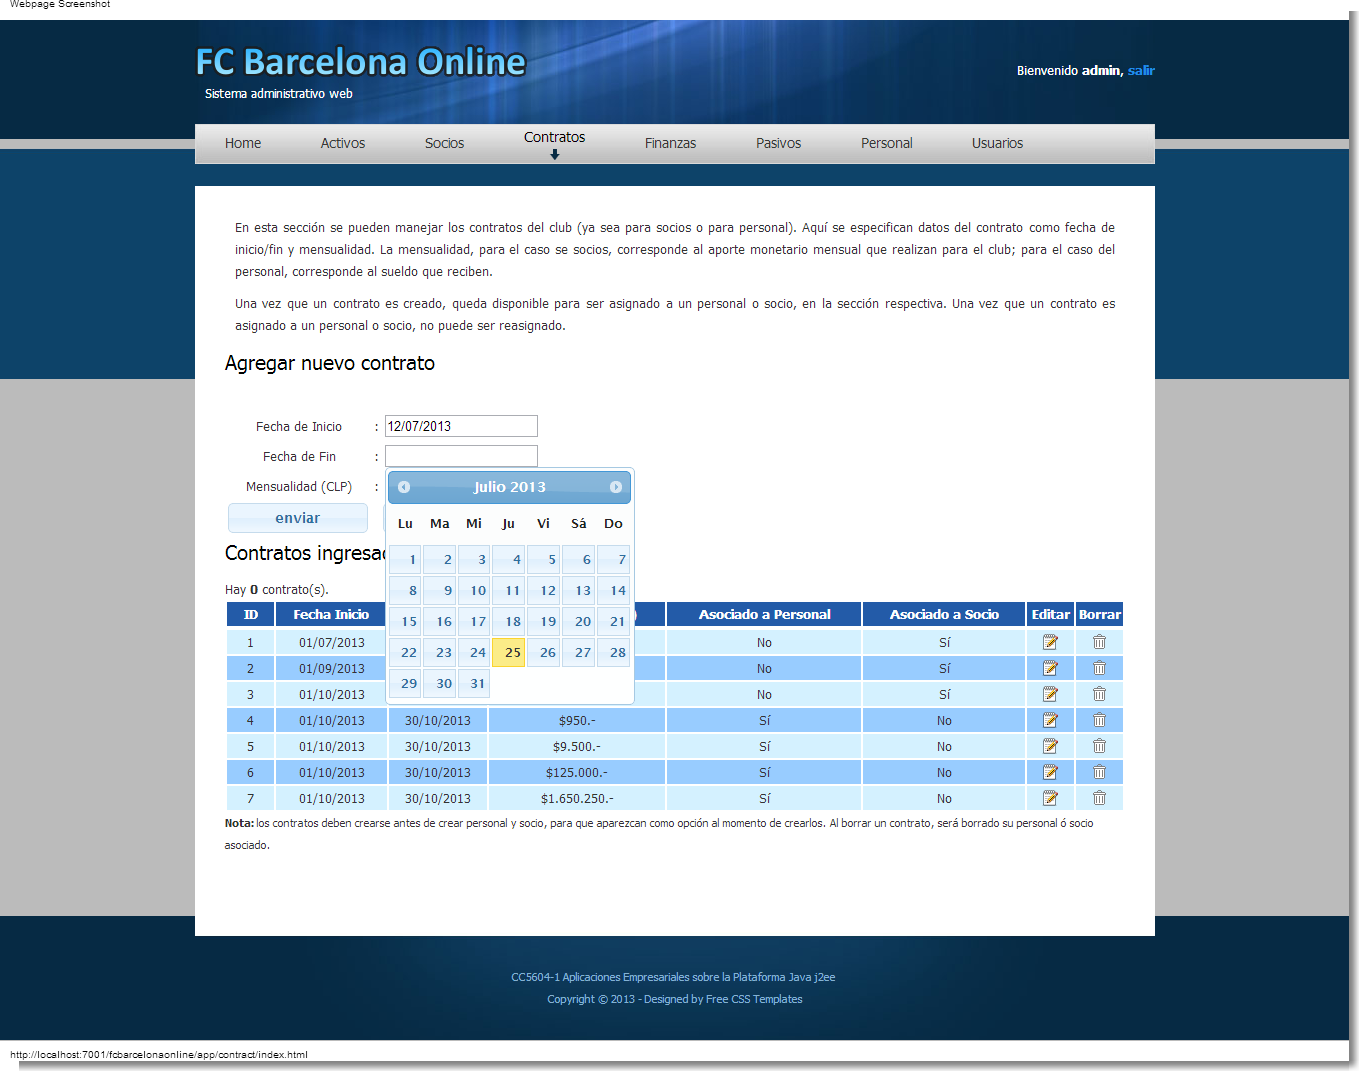
\includegraphics[width=\textwidth]{figs/fig6.png}
  \caption{Se ha utilizado Jquery-Ui para hacer la experiencia del usuario más agradable.}
\end{figure}

\begin{figure}
\centering
  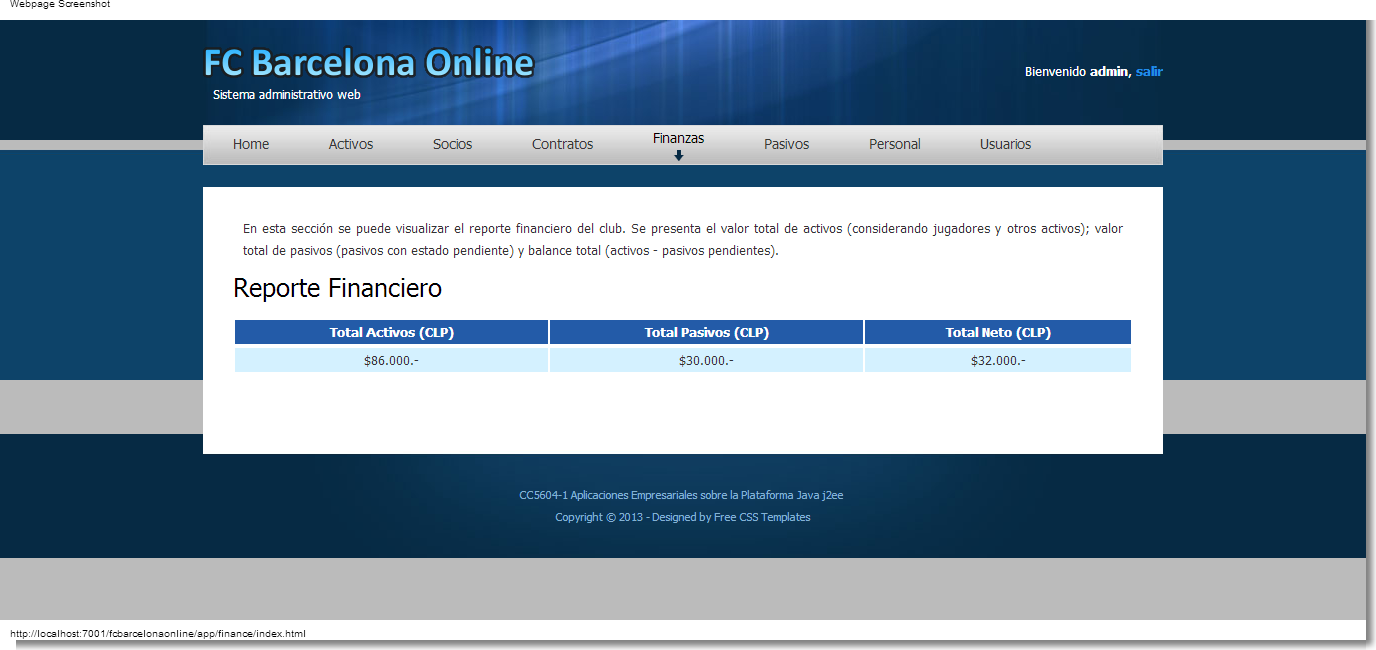
\includegraphics[width=\textwidth]{figs/fig7.png}
  \caption{Se muestra el resumen financiero del club, según lógica indicada en los requerimientos.}
\end{figure}

\begin{figure}
\centering
  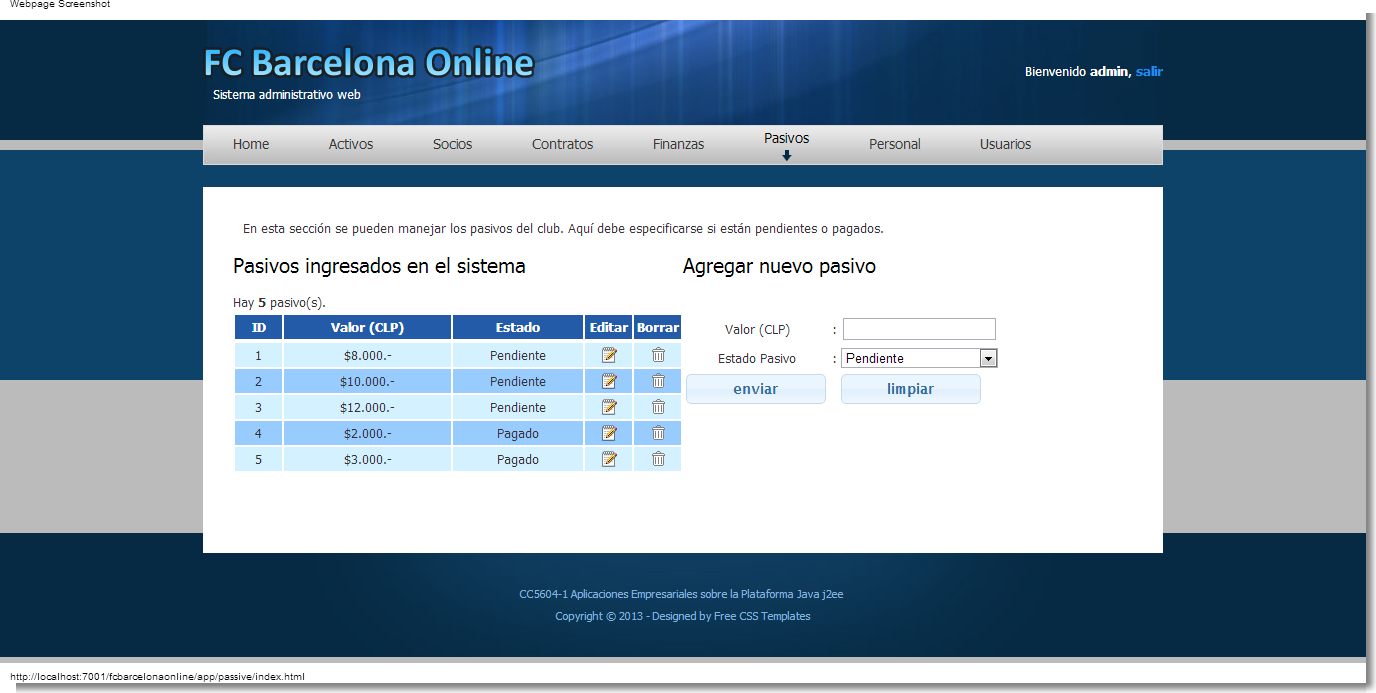
\includegraphics[width=\textwidth]{figs/fig8.png}
  \caption{Pantalla de administración de pasivos de la aplicación.}
\end{figure}

\begin{figure}
\centering
  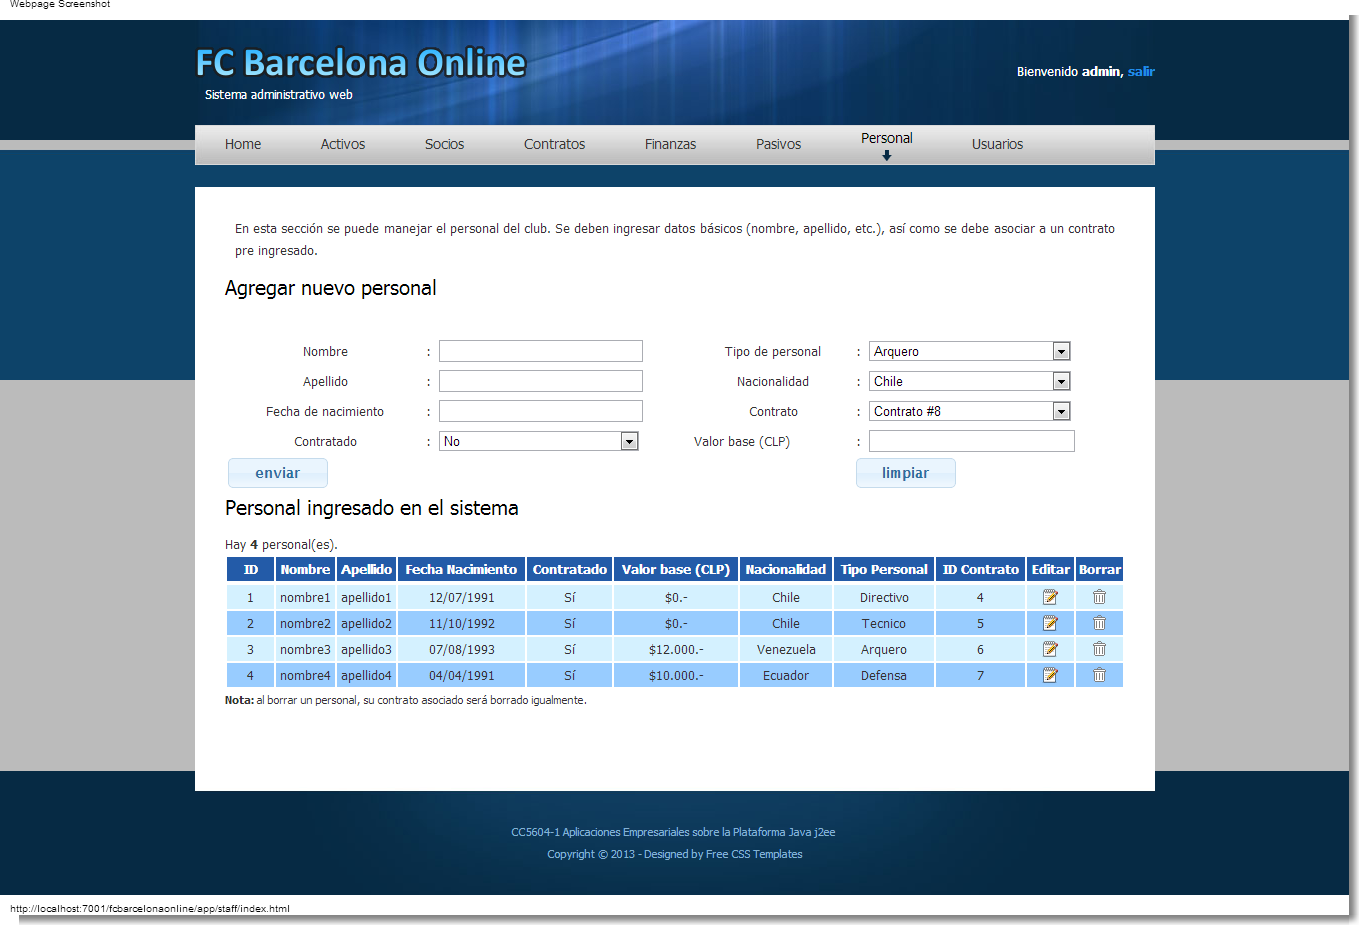
\includegraphics[width=\textwidth]{figs/fig9.png}
  \caption{Pantalla de administración de personal de la aplicación.}
\end{figure}

\begin{figure}
\centering
  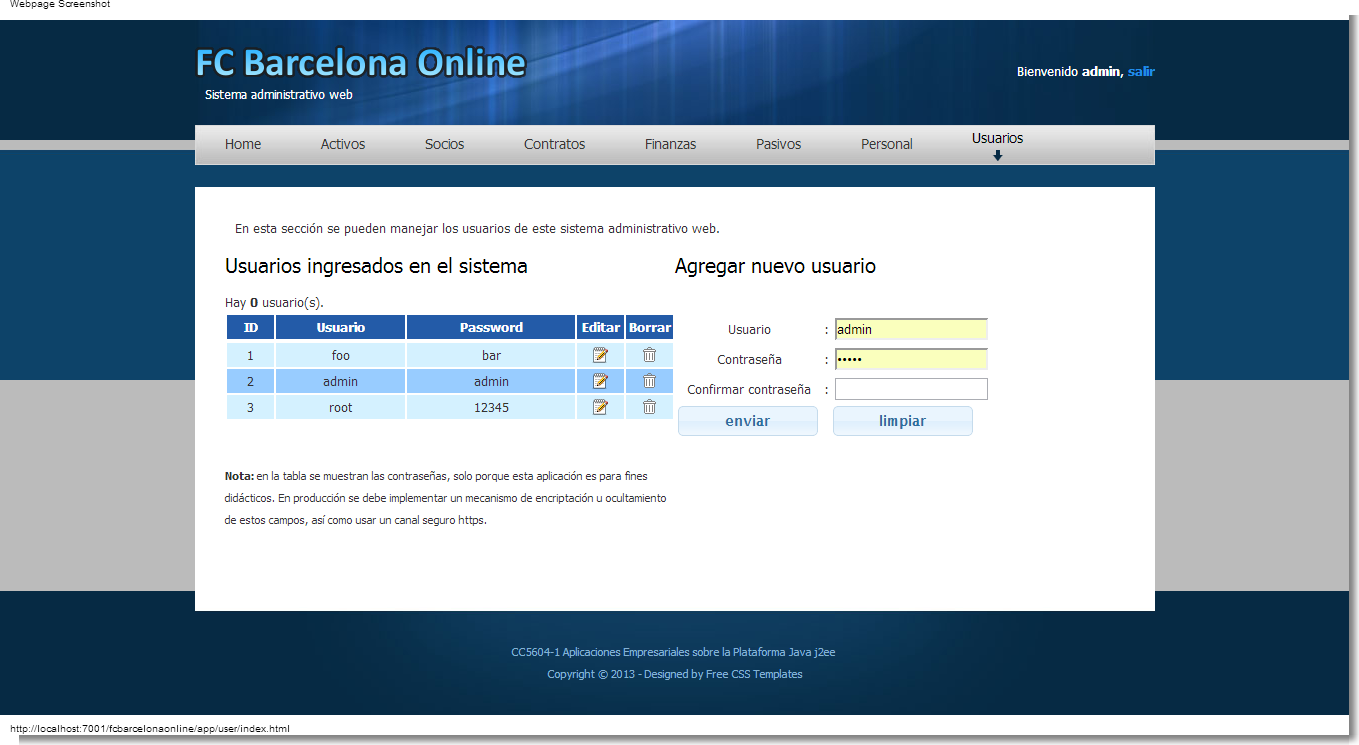
\includegraphics[width=\textwidth]{figs/fig10.png}
  \caption{Pantalla de administración de usuarios. Se ha utilizado ajax para comprobar en tiempo real la disponibilidad del nombre de usuario siendo agregado.}
\end{figure}

\subsection{Construcción y despliegue.}

Se ha creado un script para ant, altamente configurable, que permite construir la aplicación (compilar y empaquetar). Se ha seguido el mismo esquema que Intellij, para poder alternar entre uno u otro, según se necesite (por ejemplo, para debugear es mejor construir la aplicación desde el IDE, pero para producción es mejor usar ant).

En un archivo separado, se han definido las propieades y opciones para el empaquetado, como por ejemplo, nombre de directorios intermedios, archivos, etc. Los pasos que hay que seguir para compilar correctamente la aplicación son los siguientes (se editan en archivo \texttt{build.properties}):

\begin{enumerate}
\item Configurar ruta del sdk de java en línea 47 (asegurarse que no termine en /). Propiedad \texttt{sdk.path}.
\item Configurar volcado de tests a fichero en línea 52 (false: volcar por consola, true: volcar a archivo). Propiedad \texttt{test.usefile}.
\item Configurar si se correrán los tests o no como parte del empaquetamiento del archivo ear en línea 54 (false: no correr tests, true: correr tests). Propiedad \texttt{test.run}.
\item Configurar la base de datos que se usará en línea 57 (hypersonic: base de datos integrada en memoria, oracle: base de datos externa). Propiedad \texttt{database.config}.
\end{enumerate}

Dependiendo de la base de datos escogida (oracle o hypersonic) se debe modificar el correspondiente archivo \texttt{application-db-hypersonic.properties} o \texttt{application-db-oracle.properties}. Los dos archivos tienen las mismas propiedades pero cambia ligeramente su uso. Si se escoge correr los tests, estos correrán con la base de datos en memoria siempre. Luego la aplicación se empaquetará tomando el respectivo archivo .properties indicado en el \texttt{build.properties}.

La primera línea del archivo de configuración de base de datos (propiedad \texttt{database.populate}), indica si se debe rellenar la base de datos con datos iniciales de prueba. Si la BD escogida es hypersonic, entonces conviene dejarla en \texttt{true}, para poder probar la aplicación rápidamente. Si se escoge oracle, entonces el esquema indicado debe estar vacío (sin tablas) y escoger el valor \texttt{create} para la propiedad \texttt{database.hbm2ddl.auto} de \texttt{Hibernate}.

Al momento de ejecutar las pruebas de la aplicación, se recomienda usar la configuración para \texttt{hypersonic}, con la propiedad \texttt{database.populate} en \texttt{true}. De esta forma, se podrá ingresar a la aplicación usando la url por defecto \texttt{http://localhost:7001/fcbarcelonaonline/login.html} usando el usuario/password por defecto \texttt{admin}/\texttt{admin}.

Finalmente se puede compilar, testear y empaquetar la aplicación corriendo el comando ant:
\begin{verbatim}
C:/j2ee> ant -f build.xml package
\end{verbatim}

y la aplicación ear para despliegue debería aparecer bajo el directorio \texttt{out/artifacts}.

Nota: la aplicación fue desarrollada con el JDK \texttt{1.6.0\_33} de Oracle, Intellij IDEA 11.1.4, Ant incorporado de Intellij 1.8.2 y Ant externo 1.8.4, usando las librerías incorporadas en el mismo proyecto, Oracle Weblogic v12.1.1.0, navegador google Chrome Versión 28.0.1500.72 m y Windows 7 Home Premium.

\end{document}


